% Created 2013-11-12 Tue 20:00
\documentclass[12pt, a4paper]{article}
\usepackage{polski}
\usepackage[utf8x]{inputenc}
\usepackage[polish]{babel} 
\usepackage{geometry}
\usepackage{hyperref}
\usepackage{amsmath}
\usepackage[numbers]{natbib}
\usepackage{algorithm}
\usepackage{algpseudocode}
\usepackage{float}
\usepackage{graphicx}
\usepackage{listings}

\lstdefinelanguage{scala}{
  morekeywords={abstract,case,catch,class,def,%
    do,else,extends,false,final,finally,%
    for,if,implicit,import,match,mixin,%
    new,null,object,override,package,%
    private,protected,requires,return,sealed,%
    super,this,throw,trait,true,try,%
    type,val,var,while,with,yield},
  otherkeywords={=>,<-,<\%,<:,>:,\#,@},
  sensitive=true,
  morecomment=[l]{//},
  morecomment=[n]{/*}{*/},
  morestring=[b]",
  morestring=[b]',
  morestring=[b]"""
}

\author{Marek Lewandowski, Juliusz Gonera}
\date{}
\title{Porównanie algorytmów znajdowania maksymalnej kliki w grafie}
\begin{document}

\maketitle

\section{Problem maksymalnej kliki}
\label{sec-1}
Kliką nazywamy spójny podgraf, taki że nie jest on zawarty w żadnym innym spójnym podgrafie. Maksymalna klika to klika składająca się z największej liczby wierzchołków. Problem znajdowania maksymalnej kliki w grafie jest problemem NP-zupełnym.

\section{Algorytm BasicMC}
\label{sec-2}
Do zaimplementowania został wybrany algorytm \ref{basicmc} przechodzący graf w głąb i używający techniki branch-and-bound w celu znalezienia maksymalnej kliki. Algorytm został opisany w \citep{bioinf} (Fig. 2). Zostanie on porównany z dostępną implementacją algorytmu Brona-Kerboscha w bibliotece JGraphT\citep{jgrapht}.

\subsection{Struktury danych}

W algorytmie \ref{basicmc} wykorzystywane są zbiory $Q$ i $Q_{max}$. $Q$ przechowuje wierzchołki aktualnie rozpatrywanej kliki. $Q_{max}$ zawiera wierzchołki największej kliki jaką dotąd udało się znaleźć. $R \subseteq V $ zawiera listę wierzchołków które mogą zostać dodane do $Q$.

\subsection{Opis Algorytmu}

Początkowo $Q := \emptyset, Q_{max} := \emptyset, R := V$. Wybieramy wierzchołek $p$ z dostępnych wierzchołków w $R$ i dodajemy go do $Q$ \algref{basicmc}{addPToQ}. Następnie obliczamy $R_{p} := R \cap \text{adj(}p\text{)}$ który staje się nowym zbiorem wierzchołków do przejrzenia. Procedura EXPAND() jest wywoływana rekursywnie do wyczerpania zbioru wierzchołków $R_{p}$. Jeśli $|Q|+|R| \leq |Q_{max}|$ to $Q \cup R$ może zawierać jedynie klikę niewiększą od $|Q_{max}|$, w tym przypadku algorytm pomija zbędne obliczenia.\algref{basicmc}{skip}

\subsection{Warunek Stopu}

W momencie osiągnięcia $R_{p} = \emptyset$, Zbiór $Q_{max}$ jest maksymalną kliką. Jeśli $|Q| > |Q_{max}|$ zbiór $Q$ zastępuje zbiór $Q_{max}$. Po usunięciu wierzchołka początkowego $p$ z $Q$ i $R$ wybieramy go z wierzchołków pozostałych w $R$ i powtarzamy do przejrzenia wszystkich wierzchołków ($R = \emptyset$)

\subsection{Złożoność Obliczeniowa}
W grafie o $n$ wierzchołkach może być nie więcej niż $3^{\frac{n}{3}}$ maksymalnych klik. Złożoność obliczeniowa algorytmu Brona-Kerboscha wynosi $O(3^{\frac{n}{3}})$.
Jest to także dolne ograniczenie dla złożoności obliczeniowej implementowanego algorytmu. Faktyczne zachowanie algorytmu w zależności od rozmiaru grafu wejściowego zostało wyznaczone empirycznie.

\subsection{Złożoność pamięciowa}
\label{memory_complexity}

Złożoność pamięciowa implementowanego algorytmu to $O(|V|)$. Ilość pamięci potrzebnej jest wprost proporcjonalna do liczby wierzchołków grafu. Wynika to bezpośrednio z definicji i sposobu użycia zbiorów $Q$, $Q_{max}$ i $R$.

\section{Algorytm Brona-Kerboscha}

Zaimplementowany algorytm BasicMC opisany powyżej został porównany z klasycznym algorytmem Brona-Kerboscha, a konkretnie z jego implementacją udostępnianą przez bibliotekę JGraphT.

Algorytm Brona-Kerboscha wybiera wierzchołek $v$ z $P$. Dodaje $v$ do $R$ i usuwa wierzchołki nie incydentne z v ze zbiorów $P$ i $X$. Dalej wybieramy kolejny wierzchołek z nowego zbioru $P$ i powtarzamy proces. Kontynuujemy dopóki $P$ nie jest zbiorem pustym. Gdy $P$ jest pusty i $X$ jest pusty zgłaszamy znalezienie nowej największej kliki (jeśli nie jest największa to $R$ zawiera podzbiór już znalezionej kliki), zawartej w zbiorze $R$. Wtedy cofamy się do ostatniego wyberanego wierzchołka i przywracamy $P$, $R$, $X$ do stanu przed wyborem kliki, usuwamy wierzchołek z $P$, dodajemy go do $X$ i rozwijamy kolejny wierzchołek.\citep{bron-kerbosch}

\begin{algorithm}
\caption{BasicMC}\label{basicmc}
\begin{algorithmic}[1]
  
\Procedure{BasicMC}{$V,E$}
\State $Q\gets \emptyset$;
\State $Q_{max}\gets \emptyset$;
\State \Call{EXPAND}{V};
\EndProcedure
\Statex

\Procedure{expand}{$R$}
\While{$R \not= \emptyset$}
  \State $p\gets v\in R$
  \If{$|Q|+|R| > |Q_{max}|$}
    \State $Q \gets Q \cup {p}$\label{addPToQ}
    \State $R_p \gets R \cap adj(p)$
    \If{$R_p \not= \emptyset$}
      \State \Call{EXPAND}{$R_{P}$}
    \ElsIf{$|Q| > |Q_{max}|$}
      \State $Q_{max} \gets Q$
    \EndIf
    \State $Q \gets Q - {p}$
  \Else
    \textbf{ return}\label{skip}
  \EndIf
  \State $R \gets R - p$
\EndWhile
\EndProcedure

\end{algorithmic}
\end{algorithm}

\begin{algorithm}
\caption{Bron-Kerbosch}\label{bron-kerbosch}
\begin{algorithmic}[1]
  
\Procedure{BronKerbosch}{$R,P,X$}
  \If{$P$ and $Q$ are both empty}
    \State report $R$ as maximal clique
  \EndIf
  \ForAll{$v \in P$}
    \State BronKerbosch($R \cup v, P \cap adj(v), X \cap adj(v)$)
    \State $P \gets P - v$
    \State $X \gets X \cup v$
  \EndFor
\EndProcedure

\end{algorithmic}
\end{algorithm}


\section{Projekt testów}
\label{sec-4}

\subsection{Projekt Testów}
Projekt testów został podzielony na 3 części, każda odpowiedzialna za inny aspekt programu.

\subsection{Testy funkcjonane}
TODO ta sekcja powinna zostać usunięta z dokumentacji końcowej
Mają na celu pokazanie, że zaimplementowany algorytm jak i reszta aplikacji pozbawiona jest błędów. W ramach tych testów przetestowane zostaną przypadki:

\begin{itemize}
\item grafu pustego z różną liczbą wierzchołków - maksymalna klika powinna wynosić $1$
\item grafu pełnego $K_{n}$ - maksymalna klika wynosi $n$
\item grafu niespójnego zawierającego podgrafy $K_{n_{1}}$ $K_{n_{2}}$ - maksymalna klika wynosi $max(n_{1}, n_{2})$
\item grafu, które jest drzewem - maksymalna klika powinna wynosić $2$
\item kół $W_{n}$ - maksymalna klika powinna wynosić $3$
\end{itemize}

Dla pozostałej części programu - obsługi wejścia, wyjścia, opcji i innych - zostaną wykonane odpowiednie testy.

\subsection{Testy złożoności}
TODO Ta sekcja powinna zostać połączona z wynikami badaniami złożoności jako jakiś teoretyczny wstęp
\subsubsection{Złożoność pamięciowa}
Złożoność pamięciowa zostanie ustalona empirycznie na podstawie pomiarów pamięci zużytej przez program dla grafów o różnej wielkości. Oczekiwana złożoność pamięciowa programu to $O(|V|)$ (\ref{memory_complexity}). 

\subsubsection{Złożoność obliczeniowa}
Testy mają na celu empiryczne zmierzenie złożoności obliczeniowej. W tym celu zostaną wygenerowane grafy losowe z różnym prawdopodobieństwem krawędzi i różną liczbą wierzchołków. Dla każdego z wygenerowanych grafów uruchomiony zostanie algorytm. Zebrane wyniki poddane zostaną analizie statystycznej, która pozwoli określić złożoność obliczeniową.



\subsection{Testy porównawcze}
TODO ta podsekcja powinna zostać usunięta z ostatecznej dokumentacji końcowej
W celu empirycznego porównania wydajności algorytmów zostanie użyty DIMACS Benchmark Set\citep{dimacs}. Jest to zbiór nietrywialnych grafów 
dla których znana jest liczba wierzchołków tworzących maksymalną klikę w grafie.

Przed faktycznym mierzeniem czasu algorytmu dla danego grafu, algorytm zostanie uruchomiony wielokrotnie dla prostego problemu grafowego w celu ,,nagrzania'' JVM. Sam proces rozgrzewania JVM jest potrzebny do tego, aby program dawał wiarygodne wyniki, które nie są zaburzone optymalizacjami kompilatora JIT, takimi jak generowanie natywnego kodu dla często wykonywanych fragmentów kodu.

\section{TODO dokumetacja końcowa}
To co musimy zrobić to:
\begin{itemize}
\item przeredagować to co było wcześniej, tak żeby nie powtarzać tej treści 1 do 1, ale żeby najbardziej kluczowe elementy były zawarte
\item reszta TODO poniżej
\end{itemize}

\section{Artefakty projetkowe}
Razem ze sprawozdaniem dostarczone zostały następujące aretefakty projektowe:
\begin{itemize}
\item Gotowy wykonywalny program gis-maximal-clique.jar
\item Kod źródłowy programu
\item Wyniki z uruchomienia programu na grafach ze zbioru DIMACS TODO nazwa plików
\item Wyniki z testowania złożoności pamięciowej i czasowej TODO nazwa pliku
\item Automatycznie wygenerowana dokumentacja dla programisty
\item TODO coś jeszcze?
\end{itemize}

\section{Instrukcja obsługi programu}
Poniższa instrukcja powinna w kompletny sposób zapoznać użytkownika z tym jak program uruchamiać i jakie ma możliwości. Dostarczony program to typowa aplikacja CLI. Program wykonuje się na wirtualnej maszynie Javy. Program uruchamiany był na JVM w wersji 1.7. Program należy uruchamiać z linii poleceń w standardowy sposób dla programów Javowych, mianowicie:

\begin{verbatim}
java -jar gis-maximal-clique.jar
\end{verbatim}

Jako, że niektóre grafy są dość duże warto zwiększyć maksymalną ilość pamięci dostępną dla programu. 2G pamięci były wystarczające dla większości grafów ze zbioru DIMACS. Należy wtedy uruchomić program w następujący sposób:

\begin{verbatim}
java -Xmx2G -jar gis-maximal-clique.jar
\end{verbatim}

\subsection{Dane wejściowe}
Program oczekuje danych na standardowym wejściu. Danymi jest graf w formacie DIMACS. W środowisku linux korzystamy z operatora przekierowania w następujący sposób:

\begin{verbatim}
java -Xmx2G -jar gis-maximal-clique.jar < graf
\end{verbatim}

\subsubsection{Format DIMACS}

Wejściem programu są pliki tekstowe ASCII. Wejście zawiera $|E|+1$ linii nie licząc linii zawierających komentarzy. Pierwsza linijka nie będąca komentarzem jest postaci 
\begin{verbatim}
p col |V| |E|
\end{verbatim}
Gdzie $\text{p col}$ to po prostu przyjęte znaki tekstowe. $|V|$ i $|E|$ to odpowiednio liczba węzłów i krawędzi grafu. Następne $|E|$ linijek odpowiada $|E|$ krawędziom grafu. Krawędź $(v, w)$ zapisywana jest jako 
\begin{verbatim}
e W V
\end{verbatim}
i występuje tylko raz. Krawędź $(w, v)$ stanowi części reprezentacji tekstowej grafu. Podobnie jak wcześniej $e$ to zwykły znak. Opisany format jest podzbiorem formatu DIMACS opisanego w \cite{dimacs_format}

\subsection{Opcje programu}
Dostępne opcje można zobaczyć poprzez uruchomienie programu bez żadnych dodatkowych argumentów i bez podawania danych wejściowych. Opcje opisane zostały także poniżej.

\subsection{Wybór algorytmu}
Domyślnie program korzysta z algorytmu BasicMC. Aby skorzystać z algorytmu Brona-Kerboscha należy dodać argument $-j$

\subsection{Ograniczenia czasowe}
Domyślnie program działa bez ograniczenia czasowego. Mając na uwadze złożoność problemu, program może wykonywać się bardzo długo szczególnie dla dużych grafów. Można ograniczyć działanie algorytmu poprzez podanie argumentu \emph{\text{-max sekundy}} podając odpowiednią liczbę sekund.

Ograniczenie to dotyczy czasu działania \emph{algorytmu}, a nie \emph{programu}. Dla dużych grafów i krótkich czasów budowanie grafu może zająć dużo czasu, znacznie więcej niż podane ograniczenie. Ograniczenie dotyczy tylko działania algorytmu, a zatem program zakończy się po czasie nie większym niż potrzebnym na załadowanie i zbudowanie grafu dodając do tego ograniczenie w sekundach.

\subsection{Wyniki cząstkowe}
Domyślnie program wyświetla tylko najlepsze znalezione rozwiązanie. Korzystając z opcji $-progress$ program będzie wyświetlał na bieżąco kolejne najlepsze rozwiązania.

\subsection{Tylko rozmiar kliki}
Domyślnie program wyświetla etykiety wierzchołków tworzących klikę. Korzystając z opcji $-sizeOnly$ program będzie wyświetlał tylko rozmiar kliki bez wypisywania wierzchołków. Więcej informacji przy opisie formatowania.

\subsection{Formatowanie}
Domyślnie program wyświetla wyniki w poniższym formacie:

\begin{verbatim}
w(g) TIME
V1 V2 V3 ...
\end{verbatim}
Gdzie $\omega(g)$ to rozmiar największej znalezionej kliki, $\text{TIME}$ - czas wykonania algorytmu w milisekundach, $\text{V1 V2 V3}$ to etykiety wierzchołków, które tworzą klikę maksymalną. Przykładowy wynik to:

\begin{verbatim}
24 613
101 120 52 110 125 20 93 29 121 85 105 17 118 12 81 39 98 66 3 67 11 23 119 47
\end{verbatim}

Korzystając z opcji $-sizeOnly$ format wyjściowy nie będzie zawierał drugiej linijki. 

Korzystając z opcji $-csv$ program będzie wyświetlał wynik w formacie CSV z większa ilością informacji. Kolejne kolumny to:
\begin{verbatim}
Nazwa grafu, Użyty algorytm, w(g), TIME, MEMORY, CLIQUE
\end{verbatim}

gdzie $\text{MEMORY}$ to zużyta pamięć w kB, a $\text{CLIQUE}$ to numery wierzchołków podobnie jak w prostej wersji formatu. Korzystając z opcji $-sizeOnly$ wyjście nie będzie zawierało kolumny $\text{CLIQUE}$.

\subsection{Tryb benchmark}
Program można włączyć w trybie benchmark. Będzie wtedy testował dany algorytm na losowo wygenerowanym spójnym grafie nieskierowanym z zadanymi parameterami. Aby włączyć program w tym trybie należy podać argument z dwiema wartościami \emph{\text{-benchmark N p}} gdzie $N$ to maksymalna liczba wierzchołków w losowo wygenerowanym grafie, a $p$ to prawdopodobieństwo wystąpienia krawędzi. $N$ powinno być większe od 10.

Opcja benchmark łączy się tylko z wyborem algorytmu. Pozostałe argumenty są pomijane. Format wyjściowy to CSV.

\subsubsection{Działanie trybu benchmark}
W tym trybie wybrany algorytm wykonywany jest na coraz większych grafach losowych. Zaczynając od 10 wierzchołków, aż do podanego w opcji $N$ budowane są losowe grafy z prawdopodobieństwem krawędzi $p$. Na grafie mierzony jest czas wykonania oraz zużyta pamięć dla obydwu algorytmów. Dla każdego pośredniego rozmiaru algorytm wykonywany jest kilkukrotnie. Wyniki są agregowane i uśredniane. Następnie zaczyna się testowanie na większym losowym grafie, aż do osiągnięcia podanego $N$.

\subsection{Przykłady}

\begin{verbatim}
java -Xmx2G -jar gis-maximal-clique.jar -max 90 -progress -csv < data/graph
\end{verbatim}
Uruchamia program z ograniczeniem czasowym 90 sekund korzystając z algorytmu BasicMC wyświetlając wyniki pośrednie w formacie CSV dla grafu w formacie dimacs dostępnego pod ścieżką data/graph.

\begin{verbatim}
java -Xmx2G -jar gis-maximal-clique.jar -max 30 -j < data/graph 
\end{verbatim}
Uruchamia program z ograniczeniem czasowym 30 sekund korzystając z algorytmu Brona-Kerboscha dla grafu w formacie dimacs dostępnego pod ścieżką data/graph

\begin{verbatim}
java -Xmx2G -jar gis-maximal-clique.jar -benchmark 60 0.9
\end{verbatim}
Uruchamia program w trybie benchmark na losowych grafach zaczynając od liczby wierzchołków 10 aż do 60 z prawdopodobieństwem wystąpienia krawędzi 0.9 korzystając z algorytmu BasicMC.

\begin{verbatim}
java -Xmx2G -jar gis-maximal-clique.jar  -benchmark 50 0.7 -j
\end{verbatim}
Uruchamia program w trybie benchmark na losowych grafach zaczynając od liczby wierzchołków 10 aż do 50 z prawdopodobieństwem wystąpienia krawędzi 0.7 korzystając z algorytmu Brona-Kerboscha.

\section{Wprowadzenie do kodu dla programisty}
Program został napisany w języku Scala. Do sprawdozdania dołączona została automatycznie wygenerowania dokumentacja ScalaDoc, która jest bardzo podobna do JavaDocu. Poniżej zebrane zostały najważniejsze informacje o programie służące do wprowadzenia programisty w temat programu.

Program został podzielony na dwa moduły. Moduł IO i moduł grafów. 

\subsection{Moduł IO}
Moduł IO odpowiada za realizację funkcjonalności typowej dla aplikacji CLI, czyli interpretację argumentów, odczytanie wejścia, delegacji odpowiednich akcji do logiki grafów w zależności od podanych argumentów i wypisanie wyników na wyjście. Moduł IO został zdefiniowany w pakiecie \emph{app}.

\subsection{Moduł grafów}
Moduł grafów zawiera definicje generycznego funkcyjnego\footnote{a zatem niemutowalnego} grafu, implementacje niezorientowanego grafu, krawędzi, wierzchołków, algorytmów i funkcji pomocniczych. Najważniejszą funkcją jest funkcja \text{{graphs.Graph.findBiggestClique}}, która dokonuje obliczeń na grafie w wątkach działających w tle i w sposób asynchroniczny zwraca kolejne najlepsze wyniki. Użyta została tutaj abstrakcja znana z funkcyjnego reaktywnego programowania \emph{Observable}. Ze szczegółami tej abstrakcji czytelnik może zapoznać się u źródła \cite{rx}

\subsubsection{Modyfikacje biblioteki JGraphT}
W celu realizacji funkcjonalności wyników cząstkowych kod biblioteki musiał zostać zmodyfikowany. Konkretna klasa \emph{BronKerboschCliqueFinder} nie była otwarta na modyfikacje, dlatego też została przekopiowana do źródeł i zmodyfikowana. Dodana została także odpowiednia klasa w Scali opakowująca rozszerzoną klasę Javową z biblioteki tak, aby API było spójne i naturalne dla reszty programu.
Modyfikacje biblioteki znajdują się w pakiecie \emph{extensions}.

\subsection{Modyfikacje kodu}
\begin{itemize}
\item Nowe opcje, formaty wyjściowe i tym podobne powinny być dodawane do klasy \emph{app.App}.
\item Nowe algorytmy powinny być dodawane do klasy \emph{graphs.Graph}
\item Rozszerzenia do danych przechowywanych w wierzchołkach i krawędziach należy wprowadzać w odpowiednich klasach z pakietu \emph{graphs}
\end{itemize}

\subsection{API}
Szczegóły dotyczące API zawarte są w dokumentacji ScalaDoc dołączonej do sprawozdania.


\subsection{Implementacja algorytmu BasicMC}
Dzięki bogatej składni języka Scala implementacja wygląda bardzo podobnie do pseudokodu algorytmu.

\begin{lstlisting}[language=scala]  % Start your code-block

def maximalClique(g: UndirectedGraph): Set[Node] = {
    type V = Node
    var Q = Set[V]()
    var Qmax = Set[V]()

    def expand(r: Set[V]): Set[V] = {
      var R = r
      while (R.nonEmpty) {
        val p = R.head
        if (Q.size + R.size > Qmax.size) {
          Q = Q + p
          val Rp = R intersect g.adj(p)
          if (Rp.nonEmpty) expand(Rp)
          else if (Q.size > Qmax.size) {
            Qmax = Q
          }
          Q = Q - p
        }
        else Qmax
        R = R - p
      }
      Qmax
    }

    expand(g.V)
  }
\end{lstlisting}

\section{Porównanie algorytmów}
Algorytmy zostały porównane przy użyciu grafów DIMACS\citep{dimacs}. Są to na tyle nietrywialne grafy, że otrzymanie najlepszego znanego wyniku dla danego grafu zajmuje bardzo długi czas. Najlepszy znany wynik dla grafu C125.9\footnote{graf losowy z 125 wierzchołkami i prawdopodobieństwem krawędzi 0.9}  to $w(g)=34$. Aby ten wynik otrzymać algorytm BasicMC potrzebował, aż 5 godzin i 25 minut. Klikę o wielkości 33 znalazł po 15 minutach.

Zdecydowaliśmy się zatem ograniczyć czas działania algorytmów do 90 sekund na każdy problem i porównać wyniki pomijając fakt, że są one dużo gorsze od najlepszych rozwiązań.

Grafy DIMACS można znaleźć w \cite{dimacs}.

\subsection{Warunki przeprowadzonych testów na zbiorze DIMACS}
Każdy test został przeprowadzony w następujących warunkach:

\begin{itemize}
\item Program ma do dyspozycji 2G pamięci
\item Czas mierzony jest dopiero od momentu uruchomienia algorytmu, a nie programu\footnote{dla niektórych problemów grafowych, samo zbudowanie grafu trwa parę minut}
\item Algorytm zwraca kolejne coraz lepsze wyniki. Dla każdego wyniku liczony jest czas jego otrzymania.
\item Końcowym wynikiem jest najlepszy wynik otrzymany w ciągu 90 sekund.\footnote{sytuacja, w której algorytm kończy działanie przed upływem czasu jest obsługiwana, ale w praktyce dla grafów ze zbioru DIMACS nie występuje}
\item Algorytm uruchamiany jest bez rozgrzewania JVM. Każde uruchomienie jest na tyle długie, że rozgrzewanie jest zbędne.
\item Program uruchamiany był na procesorze i7 2.6GHz
\end{itemize}

\subsection{Wyniki testów dla grafów ze zbioru DIMACS}
Na początku przyjrzymy się wynikom otrzymanym dla każdego z grafów, a następnie na czas otrzymania tego wyniku. Wyniki przedstawione zostały na wykresach \ref{fig:dimacs-best-part1} i \ref{fig:dimacs-best-part2}. 

\subsubsection{Najlepsze rozwiązania}
Można zauważyć, że dla każdego grafu algorytm BasicMC daje takie same lub lepsze wyniki przy danych ograniczeniach.

\begin{figure}[H]
  \begin{center}
  \fbox{
    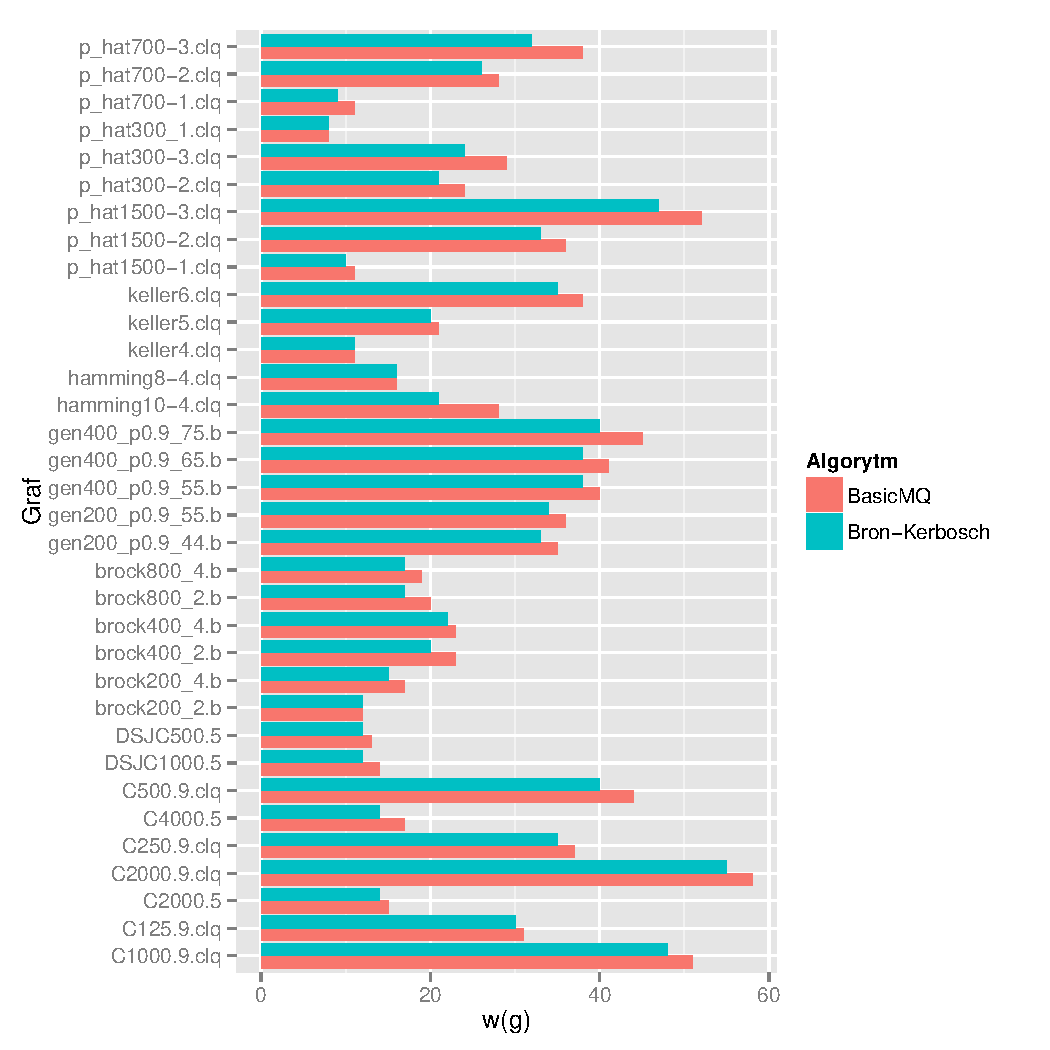
\includegraphics[width=\textwidth]{img/dimacs1.pdf}
  }
  \end{center}
  \caption{Najlepszy wynik dla grafów DIMACS w czasie 90 sekund, część 1}
  \label{fig:dimacs-best-part1}
\end{figure}

\begin{figure}[H]
  \begin{center}
  \fbox{
    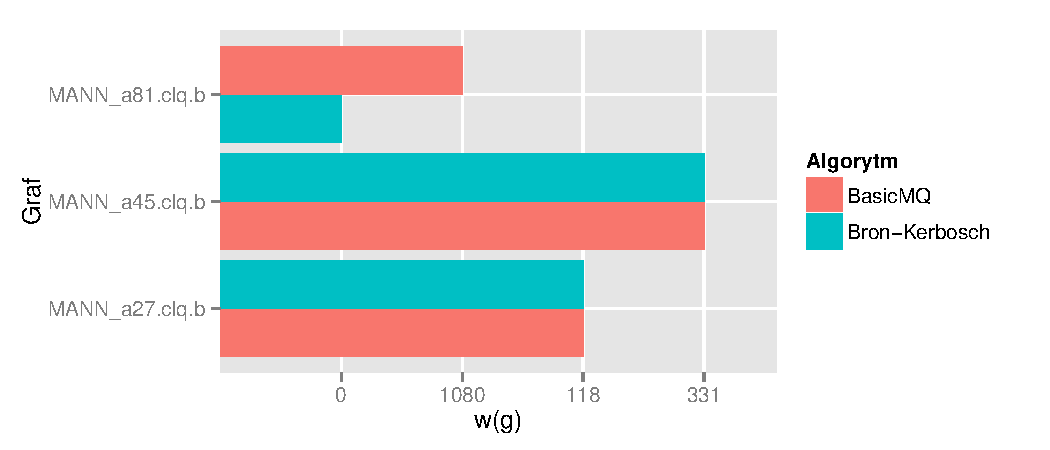
\includegraphics[width=\textwidth]{img/dimacs2.pdf}
  }
  \end{center}
  \caption{Najlepszy wynik dla grafów DIMACS w czasie 90 sekund, część 2}
  \label{fig:dimacs-best-part2}
\end{figure}

Uruchomienie algorytmu dla grafu MANN\_a81.clq dla algorytmu Brona-Kerboscha spowodowało błąd braku pamięci. Graf ten ma 3321 wierzchołków i 5 506 380 krawędzi. Test został uruchomiony ponownie z 4G pamięci. Przy ponownym uruchomieniu algorytm wykonał się poprawnie, ale nie zwrócił żadnych wyników - żadna klika nie została znaleziona w czasie 90 sekund działania algorytmu.

\subsubsection{Czas dla najlepszych rozwiązań}
TODO prawdopodobnie porównywanie czasów dla różnych najlepszych wyników to nie jest najlepsze rozwiązanie, bo gorszy algorytm czyli Bron-Kerbosch pokazuje lepsze czasy ale są to czasy dla gorszych wyników. Trzeba pobawić się trochę R i wybrać odpowiednie wyniki.

Wyniki przedstawione zostały na wykresach \ref{fig:dimacs-best-time-part1} i \ref{fig:dimacs-best-time-part2}. Na wykresie, dla niektórych grafów widzimy bardzo niskie czasy. Nie oznacza to jedak, że algorytm znalazł optymalne rozwiązanie w krótkim czasie. Oznacza to, że algorytm znalazł jedno rozwiązanie dość szybko, a potem nie mógł znaleźć żadnego lepszego rozwiązania w ciągu kolejnych 90 sekund. Dotyczy to grafów 
p\_hat300\_1.clq, p\_hat1500-1.clq, gen200\_p0.9\_44, brock200\_2.b, DSJC500. W niektórych przypadkach dotyczy to tylko algorytmu Brona-Kerboscha np. dla grafu C500.9.clq algorytm BasicMC znalazł lepsze rozwiązanie przed końcem czasu.



\begin{figure}[H]
  \begin{center}
  \fbox{
    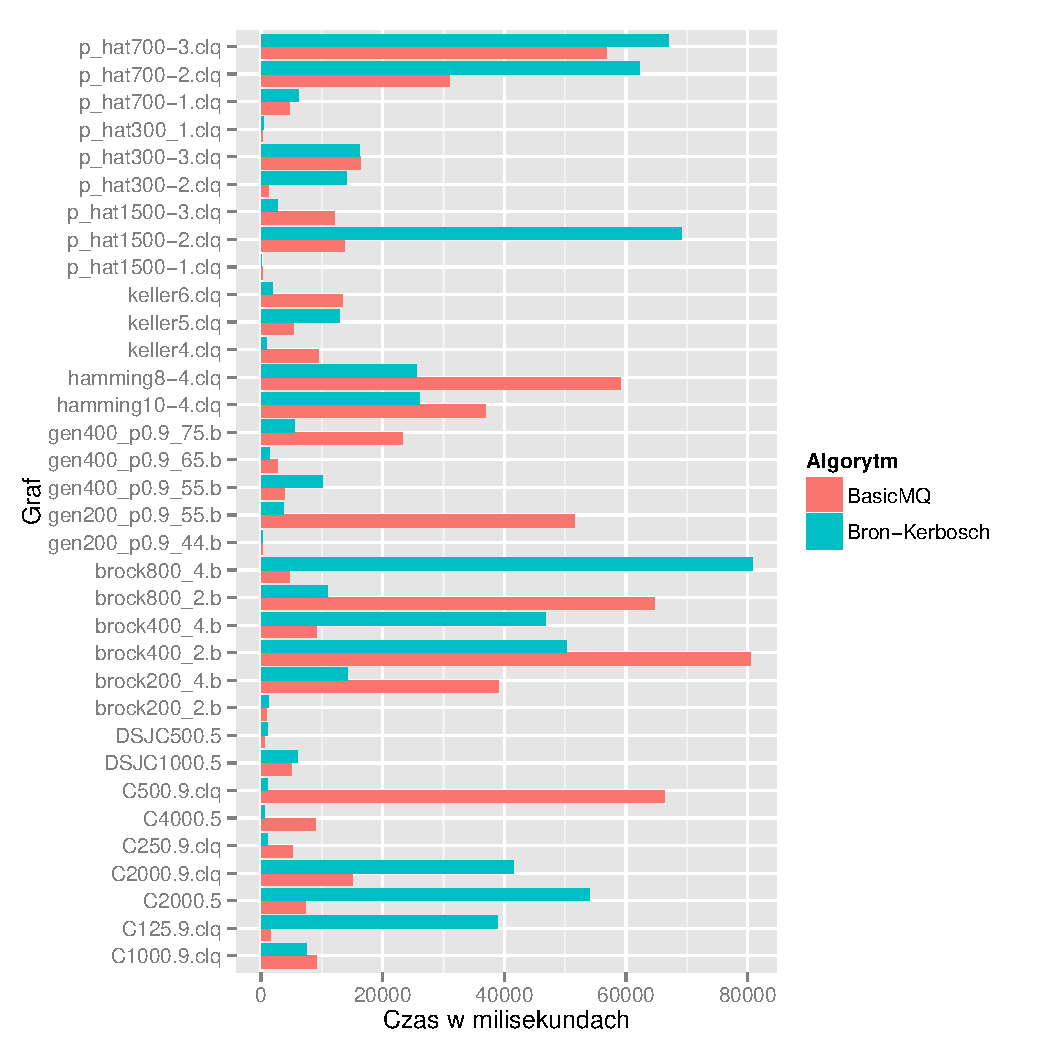
\includegraphics[width=\textwidth]{img/dimacs1czas.pdf}
  }
  \end{center}
  \caption{Czas osiągnięcia wyniku dla grafów DIMACS w czasie 90 sekund, część 1}
  \label{fig:dimacs-best-time-part1}
\end{figure}

\begin{figure}[H]
  \begin{center}
  \fbox{
    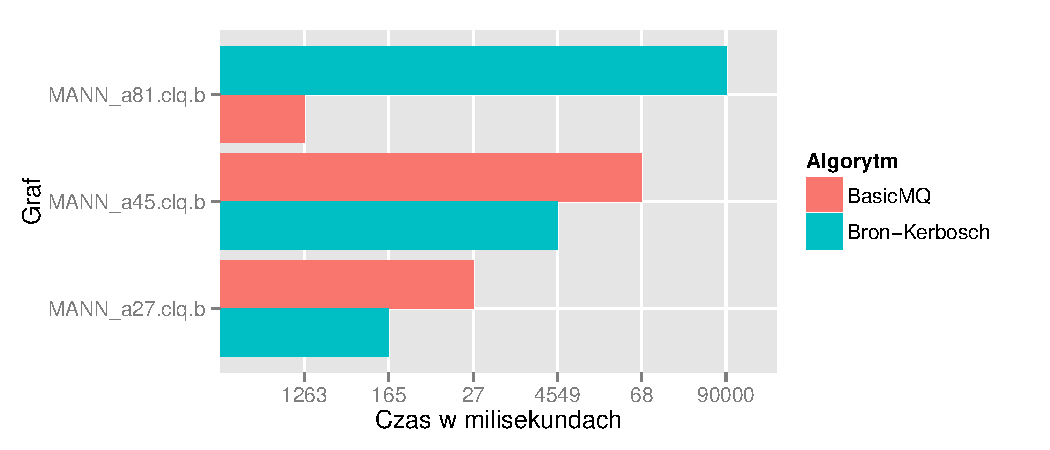
\includegraphics[width=\textwidth]{img/dimacs2czas.pdf}
  }
  \end{center}
  \caption{Czas osiągnięcia wyniku dla grafów DIMACS w czasie 90 sekund, część 2}
  \label{fig:dimacs-best-time-part2}
\end{figure}


\subsection{Szybkość znajdowania kolejnych rozwiązań}
Test ten został przeprowadzony na grafie C125.9 z ograniczeniem 20 minut. Pozostałe warunki testowe są takie same. Program uruchomiony został z opcją wyświetlania coraz lepszych wyników. Wykres \ref{fig:ProgressC125.9-20min} przedstawia wyniki tego testu. Można zauważyć kilka ciekawych rzeczy. Po pierwsze algorytm BasicMC zdążył znaleźć lepszy wynik. Najlepszy wynik znaleziony przez algorytm Brona-Kerboscha został znaleziony przez algorytm BasicMC w czasie o rząd wielkości mniejszym. Widać tutaj także regularność - BasicMC znajduje rozwiązania szybciej od algorytmu Brona-Kerboscha dla tego typu grafu.

\begin{figure}[H]
  \begin{center}
  \fbox{
    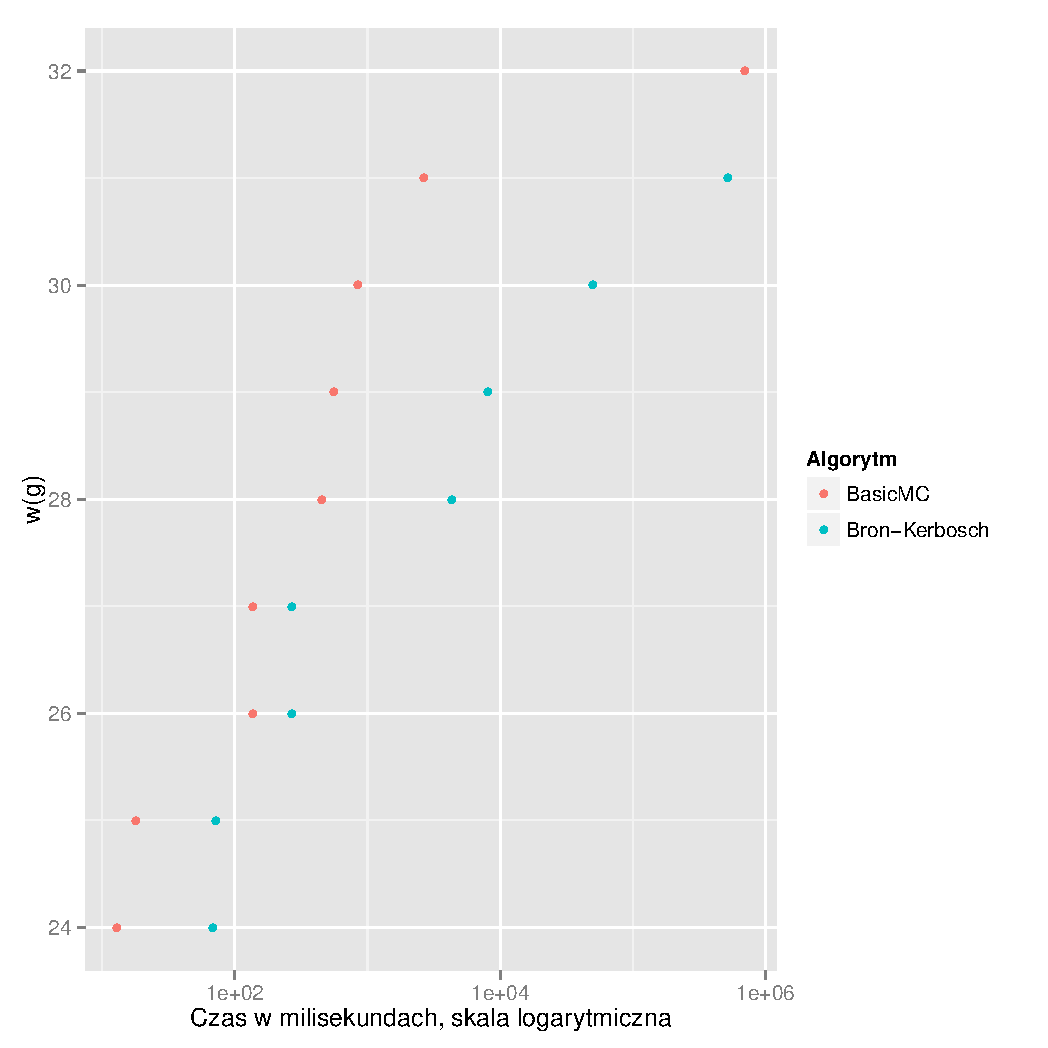
\includegraphics[width=\textwidth]{img/progress.pdf}
  }
  \end{center}
  \caption{Kolejne wyniki w czasie dla grafu C125.9 z ograniczeniem 20 minut}
  \label{fig:ProgressC125.9-20min}
\end{figure}

\section{Badanie złożoności}

Zależność czasu wykonania algorytmów w stosunku do rozmiaru grafu wejściowego została przedstawiona na \ref{fig:time-complexity}. Widać, że czas wykonania obydwu algorytmów rośnie wykładniczo w stosunku do wielkości grafów wejściowych co jest zgodne z oczekiwaniami. Warto jednak zauważyć, że algorytm BasicMC dla sprawdzonych grafów w rzeczywistości wymaga mniej czasu niż implementacja algorytmu Brona-Kerbosch biblioteki z JGraphT.

\begin{figure}[H]
  \begin{center}
  \fbox{
    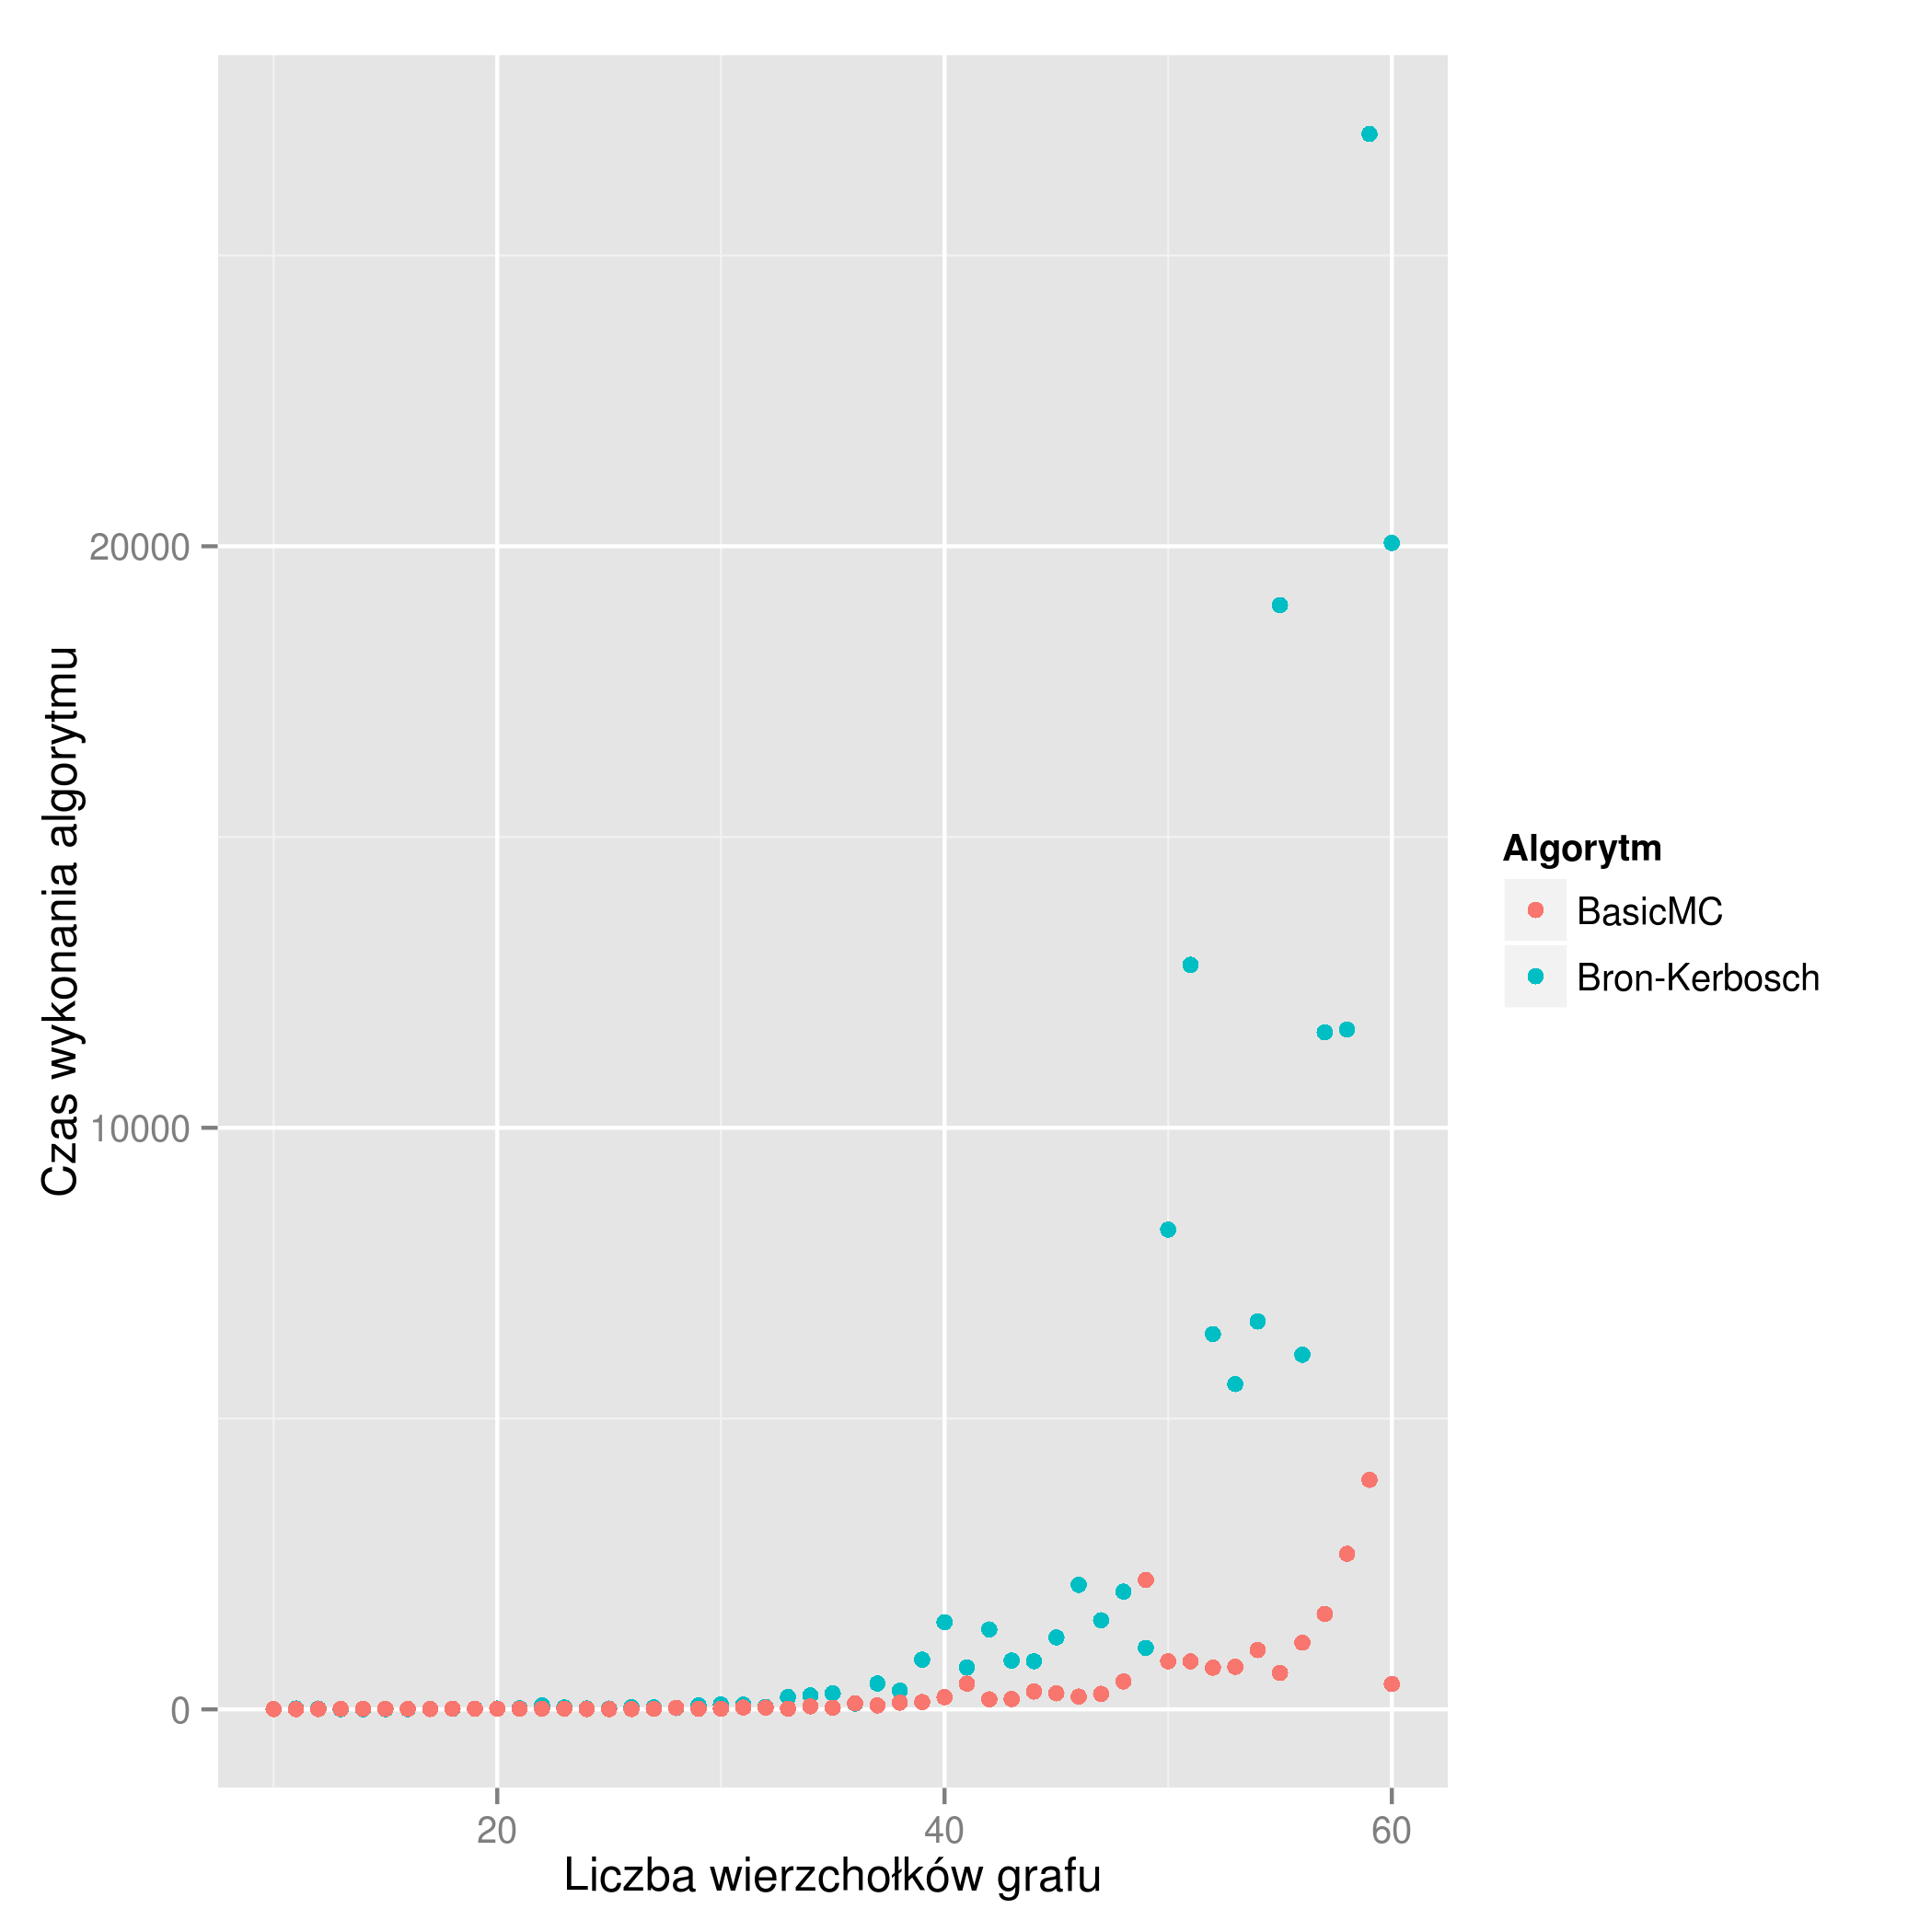
\includegraphics[width=\textwidth]{img/czas.png}
  }
  \end{center}
  \caption{Złożoność Czasowa Algorytmów}
  \label{fig:time-complexity}
\end{figure}
\subsection{Złożoność pamięciowa}
\label{memory_complexity}

Zależność pamięciowa algorytmów w stosunku do rozmiaru grafu wejściowego dla niektórych losowo wygenerowanych grafów została przedstawiona na \ref{fig:memory-complexity}. Widać, że zużywana pamiec rośnie wykładniczo w stosunku do wielkości grafów wejściowych co jest zgodne z oczekiwaniami. Punkty odstające są wynikiem działania GC.

\begin{figure}[H]
  \begin{center}
  \fbox{
    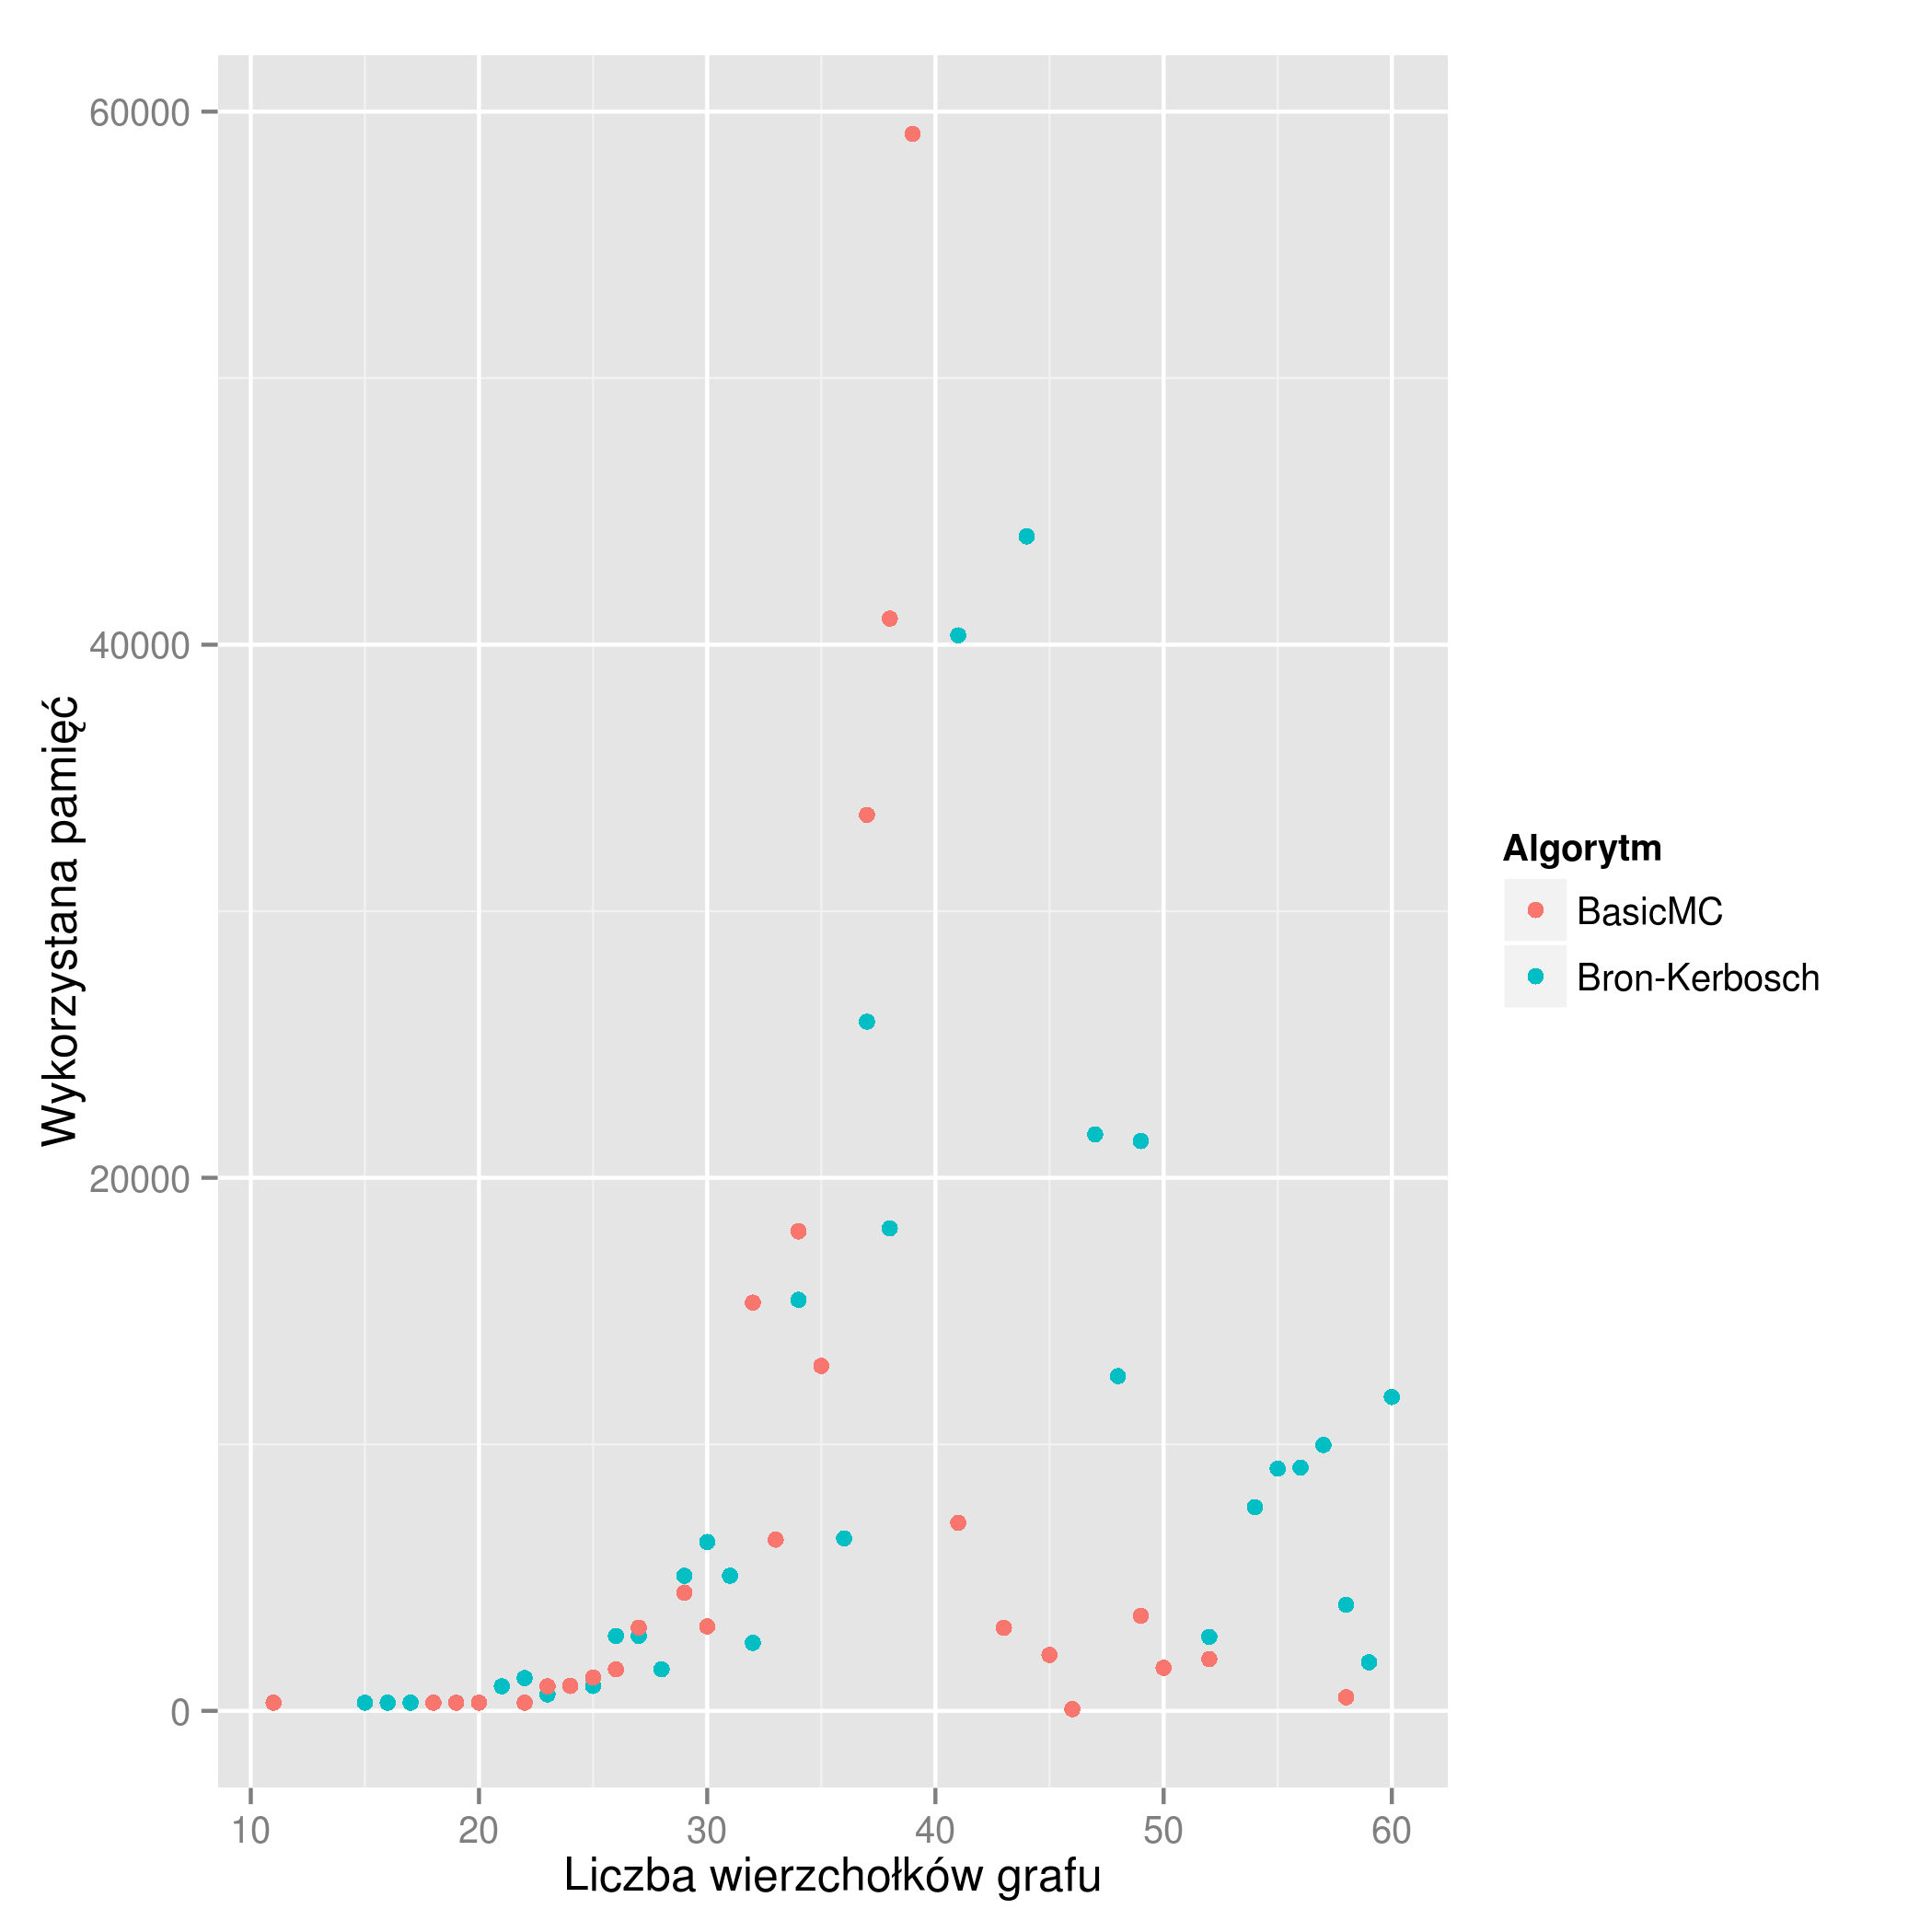
\includegraphics[width=\textwidth]{img/pamiec.png}
  }
  \end{center}
  \caption{Złożoność Pamięciowa Algorytmów}
  \label{fig:memory-complexity}
\end{figure}

\section{Testy Poprawności Implementacji}

W katalogu \textit{test/graphs/} zostały umieszczone testy podstawowych przypadków brzegowych dla zaimplementowanego algorytmu znajdowania największej kliki BasicMC.
Testy sprawdzają czy zachowane są następujące własności grafu:
\begin{itemize}
  \item maksymalna klika grafu pustego powinna mieć wielkość 1
  \item graf pełny ma maksymalną klikę wielkości równej liczbie wierzchołków
  \item cykl ma maksymalną klikę o wielkości 2
  \item graf zbudowany na cięciwach okręgu (circle graph) o liczbie wierzchołków większej niż 4 ma maksymalną klikę o wielkości 3
  \item graf zbudowany na cięciwach okręgu (circle graph) o liczbie wierzchołków równej 4 ma max. klikę o wielkości 4
  \item drzewo ma maksymalną klikę o wielkości 2
  \item graf niespójny mający dwa podgrafy $K_{n_{1}}$ $K_{n_{2}}$ posiada maksymalną klikę wynoszącą $max(n_{1}, n_{2})$
\end{itemize}

Struktura grafów użytych w testach jest generowana losowo przy każdym uruchomieniu testów.

Testy które sprawdzają, że losowo wygenerowany graf jest poprawny:
\begin{itemize}
  \item test spójności grafu - każdy wierzchołek ma conajmniej jednego sąsiada
  \item test na oczekiwaną liczbę krawędzi grafu z zadanym prawdopodobieństwem $p$ - liczba krawędzi przy prawdopodobieństwie p zawiera się w oczekiwanej liczbie krawędzi dla losowego grafu od $(p - \epsilon, p + \epsilon)$
  \item graf ma zadaną liczbę wierzchołków $n$
\end{itemize}

Aby uruchomić testy należy wykonać \textit{sbt test}\footnote{wymagany jest zatem program sbt http://www.scala-sbt.org/} w głównym katalogu programu. Pełna lista spełnianych asercji została umieszczona w sprawozdaniu \ref{fig:tests}.

\begin{figure}[H]
  \begin{center}
  \fbox{
    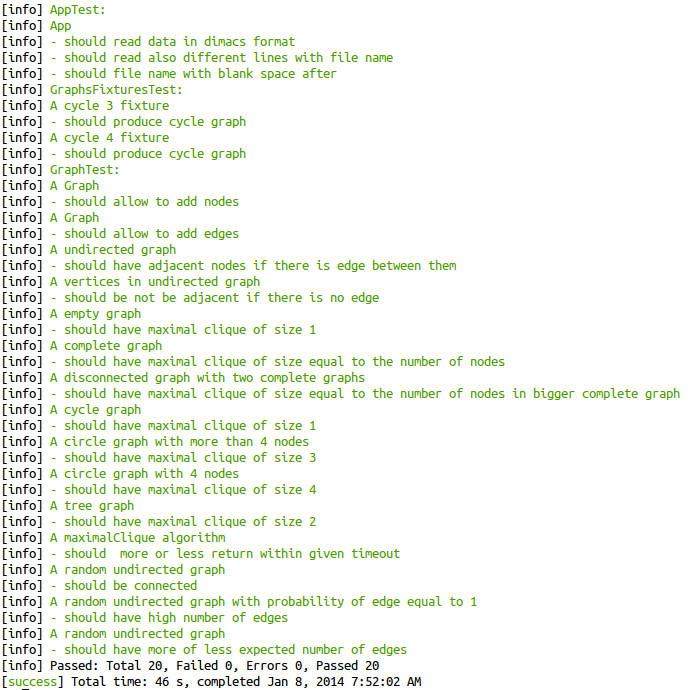
\includegraphics[width=\textwidth]{img/tests.png}
  }
  \end{center}
  \caption{Asercje spełniane przez BasicMC}
  \label{fig:tests}
\end{figure}


\section{Wnioski}

TODO tutaj będą zebrane wszystkie wnioski na temat obu algorytmów. Część informacji będzie powtórzona z poprzednich sekcji. Tutaj po prostu bedą zebrane w jednym miejscu.


\nocite{*}
\bibliographystyle{plainnat}
\bibliography{bibliography}
\end{document}
